\documentclass{beamer}
\usepackage[latin1]{inputenc}

\usetheme{Madrid}
\usecolortheme{default}
\usepackage{amsmath}
\usepackage{amssymb,amsfonts,amsthm}
\usepackage{txfonts}
\usepackage{tkz-euclide}
\usepackage{listings}
\usepackage{adjustbox}
\usepackage{array}
\usepackage{tabularx}
\usepackage{gvv}
\usepackage{lmodern}
\usepackage{circuitikz}
\usepackage{tikz}
\usepackage{graphicx}
\usepackage{gensymb}
\usepackage{physics}

\setbeamertemplate{page number in head/foot}[totalframenumber]

\usepackage{tcolorbox}
\tcbuselibrary{minted,breakable,xparse,skins}



\definecolor{bg}{gray}{0.95}
\DeclareTCBListing{mintedbox}{O{}m!O{}}{%
  breakable=true,
  listing engine=minted,
  listing only,
  minted language=#2,
  minted style=default,
  minted options={%
    linenos,
    gobble=0,
    breaklines=true,
    breakafter=,,
    fontsize=\small,
    numbersep=8pt,
    #1},
  boxsep=0pt,
  left skip=0pt,
  right skip=0pt,
  left=25pt,
  right=0pt,
  top=3pt,
  bottom=3pt,
  arc=5pt,
  leftrule=0pt,
  rightrule=0pt,
  bottomrule=2pt,
  toprule=2pt,
  colback=bg,
  colframe=orange!70,
  enhanced,
  overlay={%
    \begin{tcbclipinterior}
    \fill[orange!20!white] (frame.south west) rectangle ([xshift=20pt]frame.north west);
    \end{tcbclipinterior}},
  #3,
}
\lstset{
    language=C,
    basicstyle=\ttfamily\small,
    keywordstyle=\color{blue},
    stringstyle=\color{orange},
    commentstyle=\color{green!60!black},
    numbers=left,
    numberstyle=\tiny\color{gray},
    breaklines=true,
    showstringspaces=false,
}
\title{9.4.38}
\date{11th october, 2025}
\author{Vishwambhar - EE25BTECH11025}

\begin{document}

\frame{\titlepage}
\begin{frame}{Question}
The diagonal of a rectangular field is 60 metres more than the shorter side. If the longer side is 30 metres more than the shorter side, find the sides of the field.\\
\end{frame}

\begin{frame}{Let}
Let:\\
The shorter side of the rectangle be x\\
The longer side of the rectangle be y\\
Then the diagonal of the rectangle will be $\sqrt{x^2+y^2}$\\
\end{frame}

\begin{frame}{Given}
Given:
\begin{align}
    \sqrt{x^2+y^2}=x+60\\
    y^2-120x-3600=0\\
    -x+y=30
\end{align}
\end{frame}

\begin{frame}{Quadratic Form}
Writing equation (3) in conic/quadratic form:
\begin{align}
    \vec{x}^\top A\vec{x}+2\vec{u}^\top\vec{x}+c=0\\
\end{align}
where,
\begin{align}
    A=\myvec{0&0\\0&1}\\
    \vec{u} = \myvec{-60\\0}\\
    c = -3600 
\end{align}
\end{frame}

\begin{frame}{Parametric form}
Writing equation(4) in parametric form:
\begin{align}
    \vec{x} = \vec{p} + t\vec{m}
\end{align}
where,
\begin{align}
    \vec{p} = \myvec{0\\30}\\
    \vec{m} = \myvec{1\\1}
\end{align}
\end{frame}

\begin{frame}{Quadractic Equation}
Substituting (9) in (4), we get:
\begin{align}
    pt^2+qt+r=0\\
\end{align}
where,
\begin{align}
    p=\vec{m}^\top A\vec{m}\\
    q=2\brak{\vec{p}^\top A\vec{m}+\vec{u}^\top\vec{m}}\\
    r=\vec{p}^\top A\vec{p}+2\vec{u}^\top\vec{p}
\end{align}
\end{frame}

\begin{frame}{Sridharacharya's Formula}
By using Sridharacharya's formula,
\begin{align}
    t=\frac{1}{\vec{m}^\top A\vec{m}}\brak{-\vec{m}^\top\brak{A\vec{p}+\vec{u}}\pm\sqrt{\sbrak{\vec{m}^\top\brak{A\vec{p}+\vec{u}}}^2-\brak{\vec{m}^\top A\vec{m}}\brak{\vec{p}^\top A\vec{p}+2\vec{u}^\top\vec{p}}}}
\end{align}
Substituting (17) in (9) we get:
\begin{align}
    \vec{x}= \vec{p}+\frac{1}{\vec{m}^\top A\vec{m}}\brak{-\vec{m}^\top\brak{A\vec{p}+\vec{u}}+\sqrt{\sbrak{\vec{m}^\top\brak{A\vec{p}+\vec{u}}}^2-\brak{\vec{m}^\top A\vec{m}}\brak{\vec{p}^\top A\vec{p}+2\vec{u}^\top\vec{p}}}}\vec{m}\\
    \vec{x}= \vec{p}+\frac{1}{\vec{m}^\top A\vec{m}}\brak{-\vec{m}^\top\brak{A\vec{p}+\vec{u}}-\sqrt{\sbrak{\vec{m}^\top\brak{A\vec{p}+\vec{u}}}^2-\brak{\vec{m}^\top A\vec{m}}\brak{\vec{p}^\top A\vec{p}+2\vec{u}^\top\vec{p}}}}\vec{m}
\end{align}
\end{frame}

\begin{frame}{Conclusion}
    After substituting values in equation (18) and (19), we get:
\begin{align}
    \vec{p}_1 = \myvec{90\\120}\\
    \vec{p}_2 = \myvec{-30\\0}
\end{align}

Since the side of the rectangle cannot be negative. The correct vector is $\vec{p}_1$.\\ Therefore,
\begin{align}
    x = 90\\
    y = 120
\end{align}
\end{frame}


\begin{frame}[fragile]
    \frametitle{C Code}
    \begin{lstlisting}
#include<stdio.h>

void give_data(double *A, double *u, double *c, double *p, double *m, double *points){
    A[0] = 0; A[1] = 0; A[2] = 0; A[3] = 1;
    u[0] = -60; u[1] = 0;
    c[0] = -3600;
    p[0] = 0; p[1] = 30;
    m[0] = 1; m[1] = 1; 
    points[0] = 1; points[1] = -120; points[2] = -3600; points[3] = 1; points[4] = 30;
}
    \end{lstlisting}
\end{frame}

\begin{frame}[fragile]
    \frametitle{Python code 1}
    \begin{lstlisting}
import ctypes as ct
import numpy as np
from numpy.lib import scimath as np_scimath
lib = ct.CDLL("./problem.so")
lib.give_data.argtypes = [
    ct.POINTER(ct.c_double), ct.POINTER(ct.c_double), ct.POINTER(ct.c_double),
    ct.POINTER(ct.c_double), ct.POINTER(ct.c_double), ct.POINTER(ct.c_double)
]
pointsA = ct.c_double * 4
pointsu = ct.c_double * 2
pointsc = ct.c_double * 1
pointsp = ct.c_double * 2
pointsm = ct.c_double * 2
points = ct.c_double * 5
    \end{lstlisting}
\end{frame}

\begin{frame}[fragile]
    \frametitle{Python code 1}
    \begin{lstlisting}
A = pointsA()
u = pointsu()
c = pointsc()
p = pointsp()
m = pointsm()
data = points()
lib.give_data(A, u, c, p, m, data)
A = np.array([[A[0], A[1]], [A[2], A[3]]])
u = np.array([[u[0]], [u[1]]])
p = np.array([[p[0]], [p[1]]])
m = np.array([[m[0]], [m[1]]])
c = c[0]
    \end{lstlisting}
\end{frame}

\begin{frame}[fragile]
    \frametitle{Python code 1}
    \begin{lstlisting}
a1 = float(m.T @ A @ m)
b1 = float(2 * (p.T @ A @ m + u.T @ m))
c1 = float(p.T @ A @ p + 2 * u.T @ p + c)
D = b1**2 - 4 * a1 * c1
t1 = (-b1 + np_scimath.sqrt(D)) / (2 * a1)
t2 = (-b1 - np_scimath.sqrt(D)) / (2 * a1)
x1 = p + t1 * m
x2 = p + t2 * m
print("Intersection 1:", x1)
print("Intersection 2:", x2)
def send_data():
    return data, x1[0,0], x1[1,0], x2[0,0], x2[1,0]
    \end{lstlisting}
\end{frame}

\begin{frame}[fragile]
    \frametitle{Python code 2}
    \begin{lstlisting}
import matplotlib.pyplot as plt
from call import send_data
import numpy as np
from numpy.lib import scimath
data , Ax, Ay, Bx, By = send_data()
x = np.linspace(-30, 150, 1000)
y = scimath.sqrt((-data[1]*x)-data[2])
A = np.linspace(-30, 150, 1000)
B = -(scimath.sqrt((-data[1]*A)-data[2]))
X = np.linspace(-100, 150, 20)
Y = X+30
    \end{lstlisting}
\end{frame}

\begin{frame}[fragile]
    \frametitle{Python code 2}
    \begin{lstlisting}
plt.plot(x, y, "-r")
plt.plot(X, Y, "-g")
plt.plot(A, B, "-r")
plt.plot(Ax,Ay, "ko")
plt.text(Ax+0.1, Ay+0.1, f"({Ax:.0f},{Ay:.0f})", color = "black", fontsize = 12)
plt.plot(Bx,By, "ko")
plt.text(Bx+0.1, By+0.1, f"({Bx:.0f},{By:.0f})", color = "black", fontsize = 12)
plt.text(86.3, -115.3, r'$y^2=120(x+30)$', color = "black", fontsize = 12)
plt.text(-92.7, -60, "y=x+30", color = "black", fontsize = 12)
    \end{lstlisting}
\end{frame}

\begin{frame}[fragile]
    \frametitle{Python code 2}
    \begin{lstlisting}
plt.xlabel("X-axis")
plt.ylabel("Y-axis")
plt.grid(True)
plt.axis("equal")
plt.savefig("../figs/plot.png")
plt.show()
    \end{lstlisting}
\end{frame}

\begin{frame}{Plot}
    \begin{figure}
        \centering
        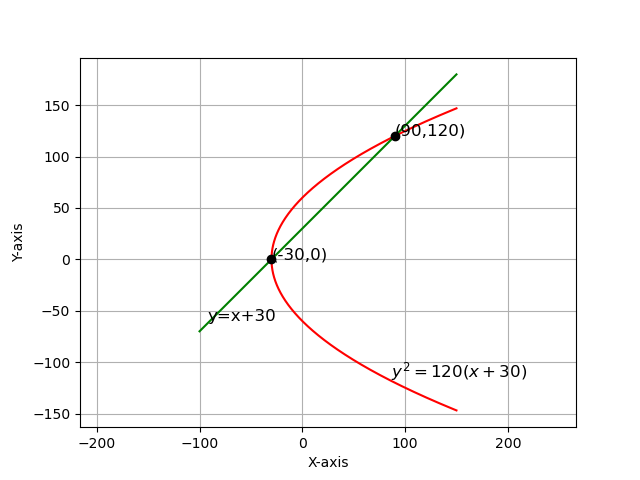
\includegraphics[width=0.5\columnwidth]{../figs/plot.png}
        \caption{Plot of the parabola and the line}
        \label{fig:fig}
    \end{figure}
\end{frame}

\end{document}